\documentclass[11pt]{article}
\usepackage{url}
\usepackage{cite}
\usepackage{amsmath}
\usepackage{amsthm}
\usepackage{graphicx}
\graphicspath{{../../umlet/}}
\graphicspath{{../../imgs/}}

\newtheorem{definition}{Definition}
\newtheorem{theorem}{Theorem}
\newtheorem{notation}{Notation}

\begin{document}

\title{Writeup}
\author{Ernest Kirstein}
\date{January 18, 2015}
\maketitle

I put together a minimal example of the the system I'll use to compile
natural language questions into SPARQL queries. This writeup will describe
the current iteration and how I hope to proceed.

\section*{Minimal Example}

Below, Figure \ref{fig:minimal} show the usage of the script 'author\_prob\_example.py'.
That's the script where I implemented the minimal example. 

\begin{figure}[h!]
    \centering
    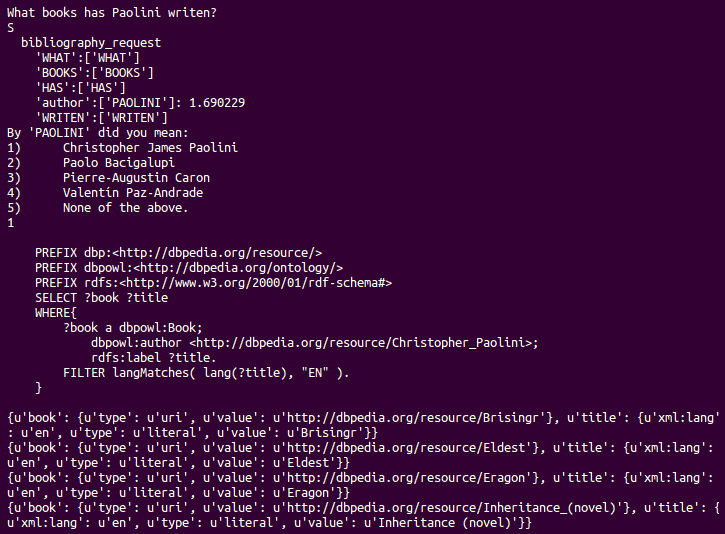
\includegraphics[width=0.9\textwidth,natwidth=1,natheight=1]{minimal_example.png}
    \caption{Using 'author\_prob\_example.py'}
    \label{fig:minimal}
\end{figure}

The script uses my own parser to recognize questions of the form,
"What books has \{author\} writen?" The name of an author is recognized based on
two pre-compiled statistical models; a distribution of the lengths of author names
and a psudo Markov-chain like model based on character N-grams. From there,
the parser approximates the probability of each possible interpretation of the
question (in this case, there can be only one) and the user can be asked to choose
from a list of the most probable interpretations. Such statistical models will
need to be compiled for each type of named entity that needs to be parsed.

Next, the chosen interpretation goes into a SPARQL generator.
The first step of SPARQL generation is to choose the particular
query type that is indicated by the top level of the parse-tree (output of the
parser).

The second query-generation step is to resolve the name of the author 
into the RDF URI which best corresponds with that natural name. 
If there are multipl close-ish names (based on the same N-gram model the parser
uses), the script asks the user which author one they meant.

Finally, the query is produced using the python mini-formatting language to fill
in a template query. This isn't very robust and will be improved on in further
iterations. With the compiled query, the script uses the SPARQLWrapper 
library to execute it.

\section*{Moving On}
The way I see it, there's three things I really need to do in the code:
\begin{itemize}
\item Make the script recognize some more complex questions. \\
    The parser can handle some really complicated stuff, and I should make that clear
    in the demo.
\item Clean up the architecture. \\
    I wiped the demo script together really quickly and it's a mess. I'm going to
    have trouble moving forward unless I take some time to clean up the high level
    structure of the code a bit.
\item Create a better interface. \\
    I'd like to create a decent interface. This isn't such a high priority so it'll
    probably have to wait. But it's something to keep in mind.
\end{itemize}

I also need to start working on the paper. I think the place to start with that is
reading more source material. Much of the work I've done already has been my own,
but I've kindof neglected the research part of this thesis. I'd like to thoroughly
understand at least a few key papers and at least scan the books you have on
natural language parsing.

%\bibliography{writeup_20150118}{}
%\bibliographystyle{plain}
\end{document}
